% !TeX spellcheck = en_GB
% !TeX root = Report.tex
\phantomsection
\addcontentsline{toc}{subsection}{Lecture 3 - Iain Gavin \& Amazon Web Services: HAILO}
\subsect{Lecture 3 - Iain Gavin \& Amazon Web Services: HAILO}

\inote{Spell checker is up the creek, all my sections need checking}
Amazon is, without any reasonable doubt, an established company.
Founded by Jeff Bezos in 1994 as an online bookshop the company shipped their first book in July 1995~\cite{seattle}.
The company now has three different parallel business interests.
The original retail aspect, a 3$^{rd}$ party selling service via the website and Amazon Web Services (AWS).
AWS powers the other two aspects of the business by providing the infrastructure that enables such excellent customer service but also acts as an accelerator for other businesses by removing the requirement for on-premises IT solutions.
They achieve this by maintaining large sever farms from which computing power can be \emph{rented} to facilitate the IT needs of a company.
They also provide varying degrees of cloud based storage; subject to access latency.

<<<<<<< HEAD
AWS considers a typical split in effort toward a computing heavy buiness venture, with an on-premises IT solution, to be $30$\% towards the actual business and $70$\% towards IT overheads~\cite{gavin2014ams}. 
Their goal is to flip this distubution by providing the infrastructe for the business. 
One such company that has acceled using AWS is Hailo~\cite{gavin2014ams}.
Launched in $2011$ with investments totalling over \$$80$ million from some well known sources; including Union Square Ventures, Accel Partners and Sir Richard Branson~\cite{hailo}.
The company maintains a smartphone app that links customers with the local taxi services however this idea is not unique.
At the time there was already a large market for smartphone enabled cab rides so something else must have been their soruce of success~\cite{ventureBeat}.
Saturation and a software only product makes patenting redundant so it must have been down to the delivering and quaility of the service that has made them a global success.
Disacotiating IT with AWS may well have been a contributing factor to their ability to concentrate on delivery.


The Amazon group as whole is very technology driven and considers innovations as the best method to drive down the prices of the products they sell.
Reasoning behind this idea is shown in Figure~\ref{fig:ScaleInnovation}.
This cycle enables price reduction which natrually improves the sales.
The key step is providing the technology which can improve the effciency therefore staying ahead of competitors.
Amazon keep delivering the required technology and at the end of $2013$ created another media buzz by publishing a patent for ``anticipatory package shipping''~\cite{spiegel2013method}! 

\inote{Need to sexify}


\begin{figure}
	\centering
	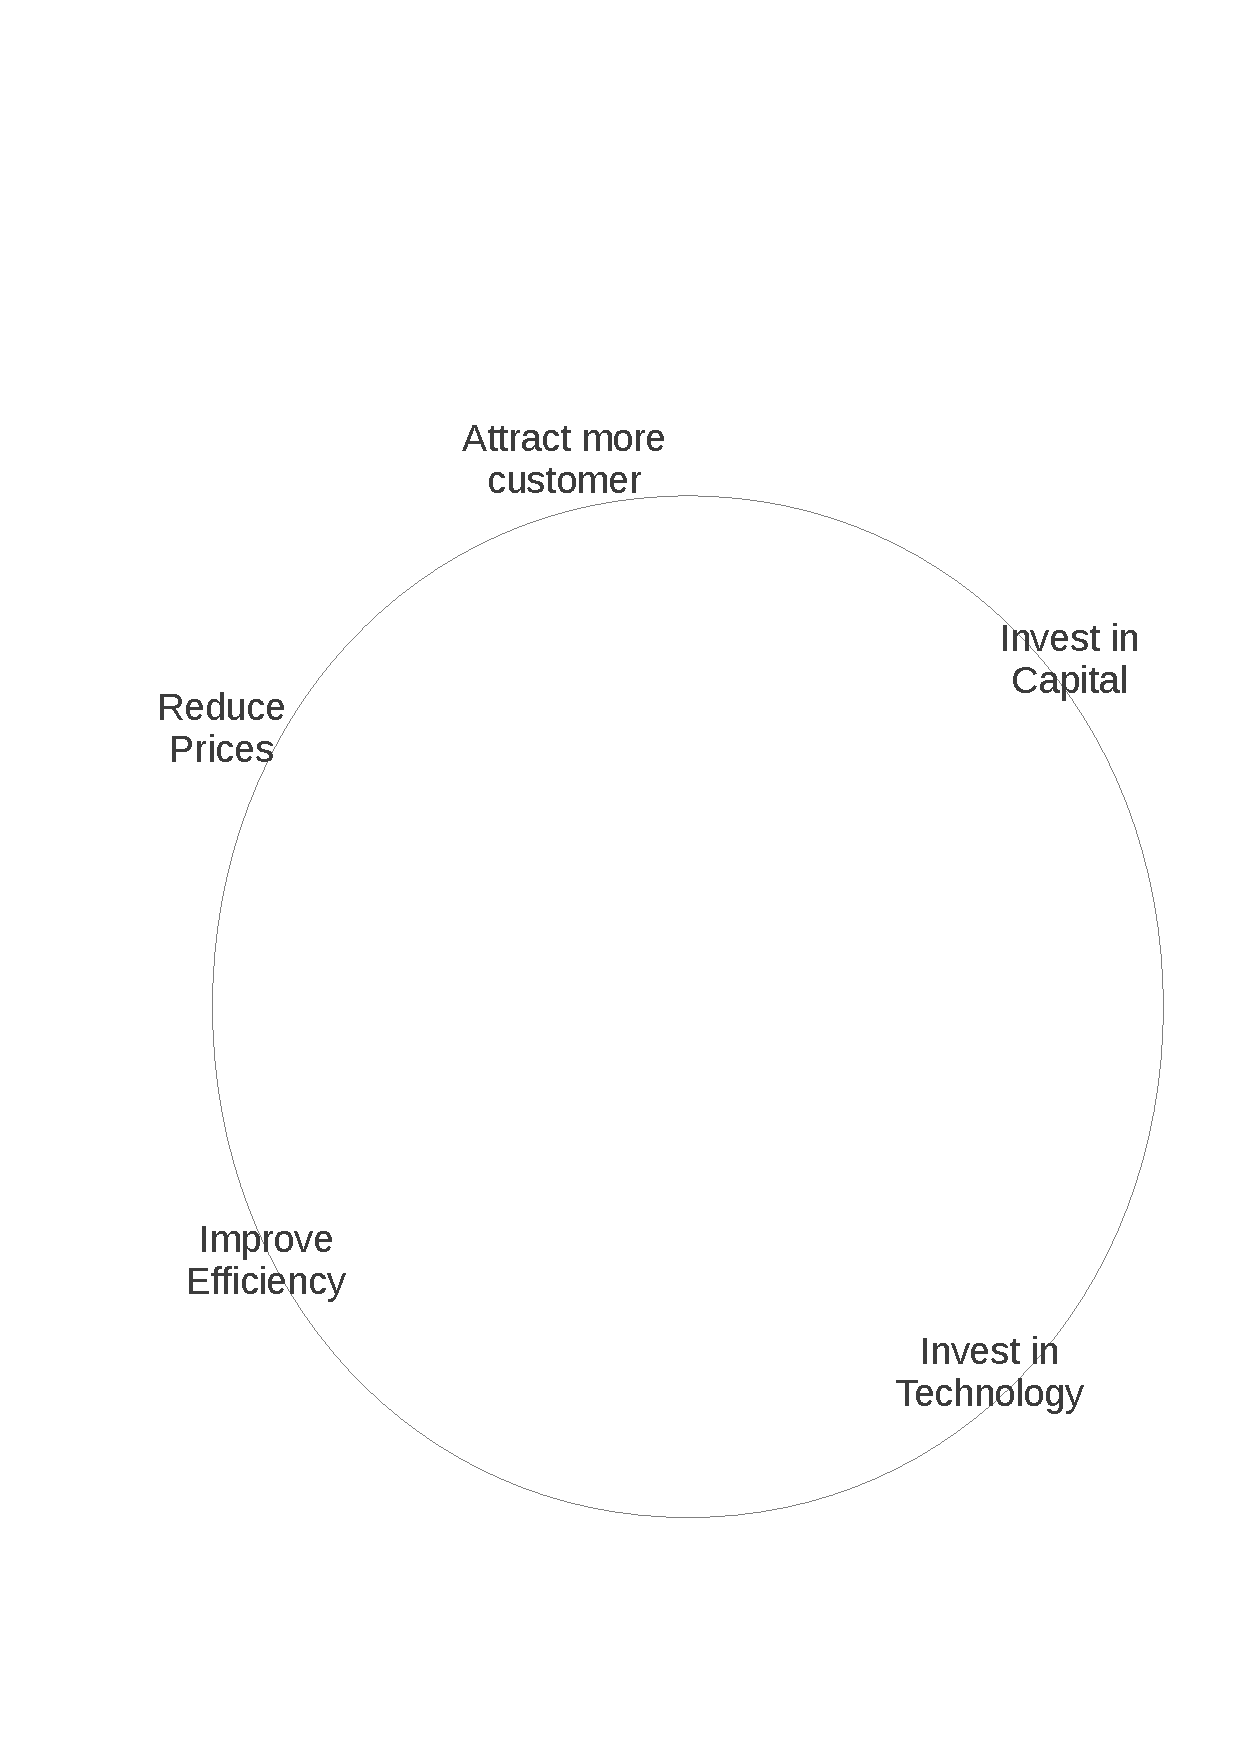
\includegraphics[width=0.5\textwidth]{./Figures/ScaleInnovation.pdf}
	\caption{Scale \& Innovation Drives Down Costs. Taken from~\cite{gavin2014ams}.}
	\label{fig:ScaleInnovation}
\end{figure}

